\chapter{机器人系统框架总体设计}
\section{机器人功能需求分析}
对于面向变电站辅助作业的运维机器人，为满足其特殊应用场景对可靠性、高性能的综合要求结合其工作内容，要求机器人具备以下功能：
（1）具备环境感知模块，可通过传感器与周围环境进行信息交互，感知自身作业环境；
（2）具备实时处理复杂空间信息的能力，实现高精度环境地图构建，以及在动态环境中的厘米级自我定位。
（3）具备基于先验地图自主导航模块，导航过程中能够自主规划出从当前位置到目标点的最优全局路径。
（4）具备任务执行过程中的未知障碍物规避能力，即在遵循全局路径的同时，实时感知并绕开未预见的障碍，并在必要时触发路径重规划机制以应对复杂的突发状况。
\section{机器人系统方案设计}
针对第~2.1节提出的环境感知、定位建图、自主导航与动态避障四项功能需求，本文采用”感知--决策--执行”的分层模块化方案设计运维机器人系统。整体方案在逻辑上划分为感知层、决策层和执行层三个层次，在物理上对应传感器模块、中央控制模块、底层运动控制模块和电源模块四类硬件，并以中央控制模块为核心实现各层之间的数据流转与指令下发。系统总体方案如图~\ref{fig:系统总体方案}所示。

\begin{figure}[!htb]
	\centering
	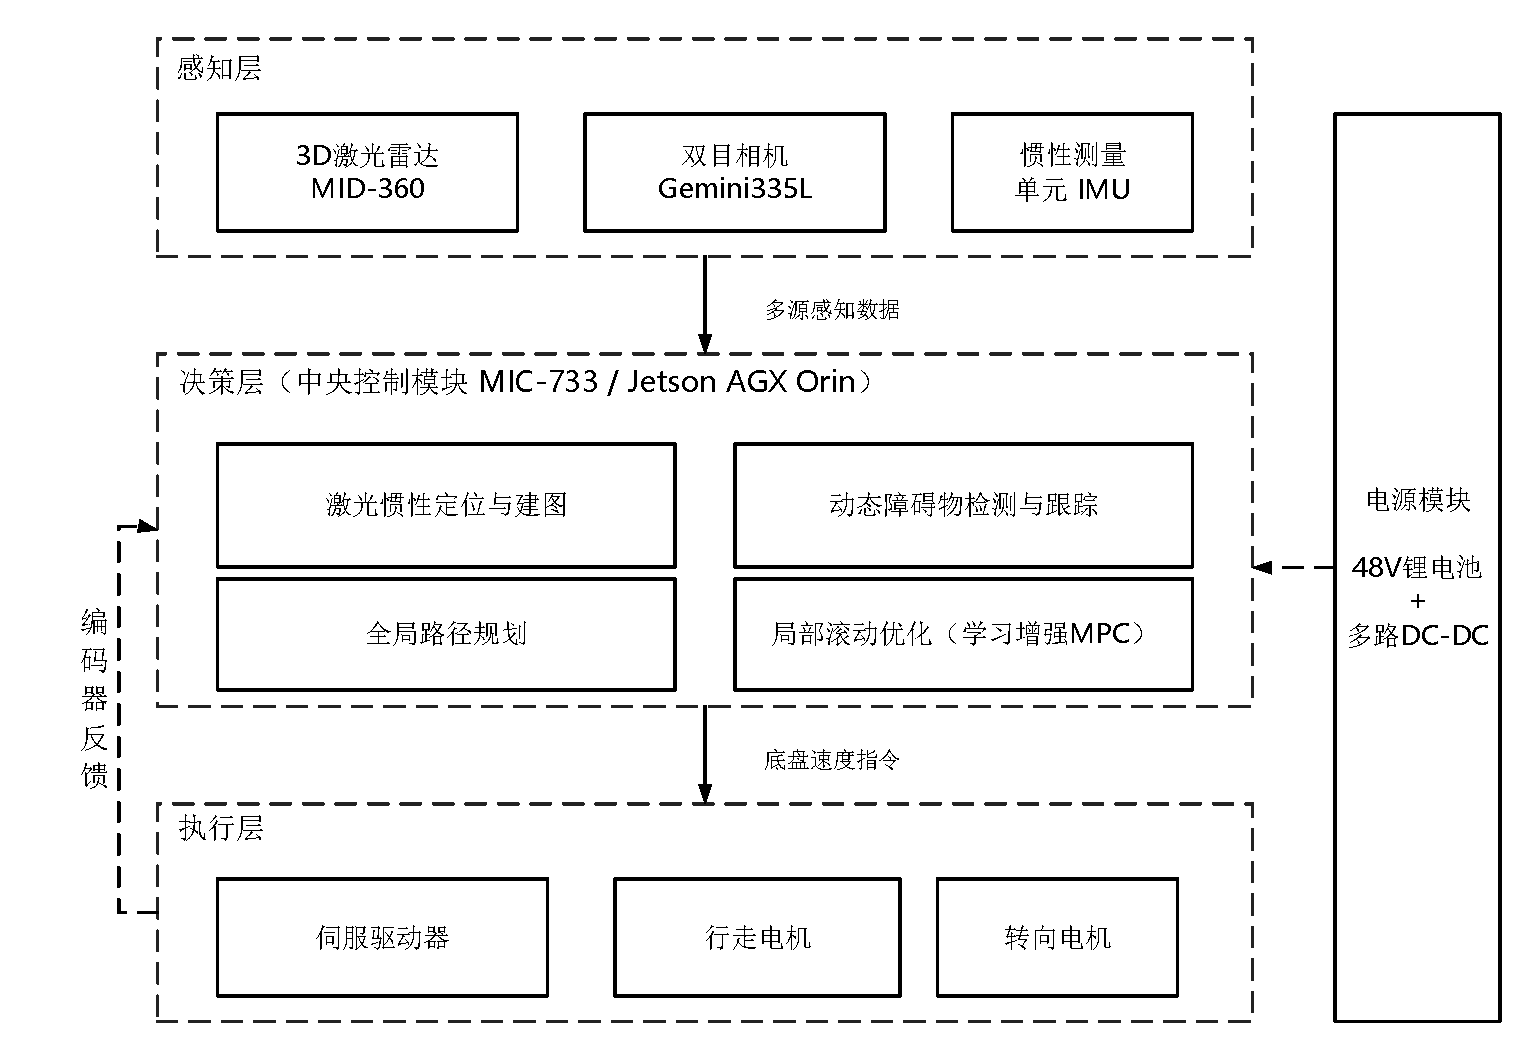
\includegraphics[width=0.95\textwidth]{pic/系统总体方案.pdf}
	\caption{机器人系统总体方案}
	\label{fig:系统总体方案}
\end{figure}

感知层位于系统底端，负责将物理环境转化为可计算的数字信息。该层由3D激光雷达、双目相机及雷达内置惯性测量单元（IMU）构成：激光雷达提供周围环境的三维点云，用于定位建图与障碍物几何提取；双目相机提供RGB图像与深度图像，用于工作目标识别与近场障碍感知；IMU提供高频角速度和加速度测量，为激光惯性里程计提供运动预测。各传感器以统一时间基准采集数据，经标准接口上传至中央控制模块。

决策层是系统的运算核心，由搭载高性能嵌入式计算平台的中央控制模块承担。该层订阅感知层上传的多源数据，依次完成激光惯性定位与地图构建、动态障碍物检测与跟踪、全局路径规划与局部滚动优化等任务，最终解算出满足运动学约束与避障要求的速度指令。考虑到激光点云配准、障碍物检测和模型预测控制等算法对算力的较高要求，决策层选用具备GPU并行加速能力的边缘计算平台，以保证导航算法的实时性。

执行层位于系统顶端，负责将决策层输出的速度指令转化为机器人的实际运动。该层由伺服驱动器、驱动电机和转向电机组成，通过CAN总线接收速度或位姿指令，驱动底盘按期望线速度和角速度运动，并将编码器反馈的实时转速、转角回传至中央控制模块，形成闭环控制。电源模块为上述各层提供稳定的多路供电，是系统持续可靠运行的能量基础。

上述分层方案使各模块职责清晰、接口规范，便于功能扩展与故障定位。下文将分别从硬件平台架构和软件系统架构两方面，对该方案的具体实现进行详细说明。

\section{机器人硬件平台架构}
\subsection{硬件选型}
机器人硬件结构包括传感器模块、中央控制模块、底层运动控制模块以及移动电源。传感器模块负责采集环境信息发送给中央控制器;
中央控制器处理传感器数据，计算出机器人运动控制指令并发送给底层运动控制模块；底层电机和舵机接受控制指令驱动机器人一定速度运动或变换到指定位姿。

\subsubsection{传感器模块}
传感器模块包括两部分：激光雷达和双目摄像头。3D激光雷达选用大疆览沃的MID-360，该激光雷达是4线束非重复扫描固态激光雷达，
由于体积小、重量轻、视场较大、分辨率较高，因此被广泛部署使用在机器人、割草机、无人车、工业和教育等智能产品中。
内部集成了IMU芯片（3轴加速度计和3轴陀螺仪），可结合点云数据构建高精地图并实现自主定位过程中的雷达坐标系、机器人坐标系、世界坐标系三者之间的转换关系。
激光雷达具体尺寸图如图~\ref{fig:Mid-360具体尺寸}所示，其性能参数如表~\ref{tab:mid360_params_centered}所示。

\begin{figure}[!htb]
	\centering
	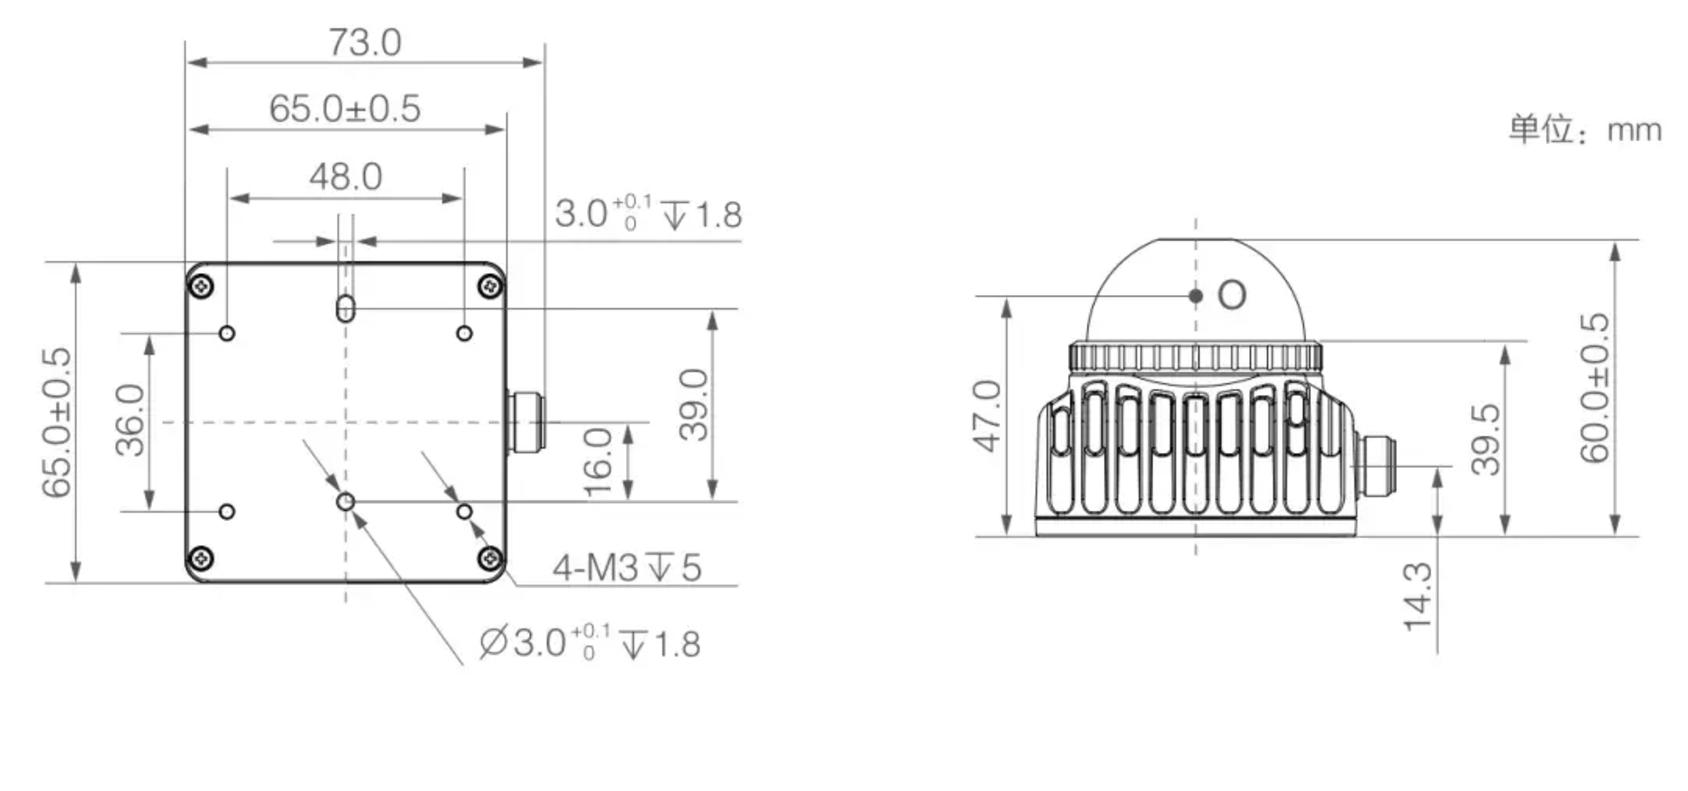
\includegraphics[width=\textwidth]{pic/激光雷达具体尺寸.pdf}
	\caption{激光雷达具体尺寸}
	\label{fig:Mid-360具体尺寸}
\end{figure}


\begin{table}[htbp]
  \centering
  \caption{MID360激光雷达性能参数}
  \label{tab:mid360_params_centered}
  \renewcommand{\arraystretch}{1.5} % 增大行间距
  \begin{tabularx}{\textwidth}{>{\centering\arraybackslash}X c c c c >{\centering\arraybackslash}X}
      \toprule[1.2pt]
      \textbf{项目} & \textbf{最小值} & \textbf{典型值} & \textbf{最大值} & \textbf{单位} & \textbf{备注} \\
      \midrule
      测距范围 & 0.1 & 10 & 40 & m & 100klux照度 \\
      测距精度 & - & ±5 & - & cm & 90\%反射率 \\
      水平视场角 & - & 360 & - & ° & 全向扫描 \\
      垂直视场角 & -7.0 & - & 52.0 & ° & - \\
      扫描模式 & - & 非重复扫描 & - & - & - \\
      虚警率 & - & <0.01\% & - & - & 100klux照度 \\
      工作温度 & -20 & - & 55 & °C & - \\
      工作电压 & 9 & - & 27 & V DC & - \\
      功耗 & - & 11 & - & W & 典型功耗 \\
      网络接口 & - & 千兆以太网 & - & - & 支持PTP、PPS \\
      \bottomrule[1.2pt]
  \end{tabularx}
\end{table}

图像采集模块包含两个双目摄像头，选用奥比中光公司的Gemini335L型号的摄像头，输出深度图像和RGB图像。
可用于目标检测、距离检测以及3D环境构建，本课题中双目摄像头主要用于移动机器人移动过程中对工作目标的识别。
双目摄像头参数见表~\ref{tab:gemini335l_params_adjusted}所示。
\begin{table}[h]
  \centering
  \caption{双目摄像头 Gemini335L 性能参数} 
  \label{tab:gemini335l_params_adjusted}
  \renewcommand{\arraystretch}{1.5} % 增大行间距
  \begin{tabularx}{\textwidth}{>{\centering\arraybackslash}X >{\centering\arraybackslash}X}
      \toprule[1.2pt] % 加粗顶线
      \textbf{规格参数} & \textbf{数值} \\
      \midrule
      最大工作范围 & 0.17-20m \\
      推荐工作范围 & 0.25-6m   \\
      基线        & 95mm         \\
      视场角      & 90°×65° @ 2m（1280×800）      \\
      分辨率      & 1280×800 @ 60fps         \\
      供电建议    & DC 5V \& $\geq$1.5A \\
      平均功耗    & < 3W \\
      工作温度    & -10-50°C \\
      \bottomrule[1.2pt] % 加粗底线
  \end{tabularx}
\end{table}

\subsubsection{中央控制模块}
中央控制模块是机器人系统的运算核心，需在有限的体积和功耗下同时承担激光惯性定位、点云处理、障碍物检测跟踪以及模型预测控制等计算密集型任务。综合考虑算力、接口丰富度、工业级可靠性和嵌入式部署要求，本文选用研华（Advantech）公司的MIC-733边缘AI推理计算机作为中央控制模块。该计算机以NVIDIA Jetson AGX Orin微型计算机为核心，集成Arm架构CPU与Ampere架构GPU，具备强大的并行计算与深度学习推理能力，可满足点云配准和滚动优化的实时性需求。同时，其工业级设计支持宽温、宽压工作，适应变电站等复杂工业环境。MIC-733的主要性能参数如表~\ref{tab:mic733_params}所示。

\begin{table}[htbp]
  \centering
  \caption{MIC-733中央控制器主要性能参数}
  \label{tab:mic733_params}
  \renewcommand{\arraystretch}{1.5}
  \begin{tabularx}{\textwidth}{>{\centering\arraybackslash}X >{\centering\arraybackslash}X}
      \toprule[1.2pt]
      \textbf{规格参数} & \textbf{数值} \\
      \midrule
      核心模块      & NVIDIA Jetson AGX Orin \\
      内存          & 32GB / 64GB LPDDR5 \\
      存储          & 64GB eMMC 5.1，支持M.2 2280 NVMe扩展 \\
      网络接口      & 4 $\times$ 10/100/1000 Mbps 千兆以太网 \\
      USB接口       & 2 $\times$ USB 2.0，4 $\times$ USB 3.2 Gen 2 \\
      串口          & 2 $\times$ RS-232/RS-422/RS-485 \\
      扩展接口      & 2 $\times$ Mini PCIe，1 $\times$ iDoor \\
      供电类型      & AT/ATX，DC 9$\sim$36V \\
      工作温度      & 0 $\sim$ +60°C \\
      尺寸 / 重量   & 192 $\times$ 230 $\times$ 87 mm / 4.5 kg \\
      \bottomrule[1.2pt]
  \end{tabularx}
\end{table}

MIC-733提供4个千兆以太网口，其中一个用于连接MID-360激光雷达并支持PTP时间同步，保证点云与IMU数据的时间一致性；USB 3.2接口用于连接双目相机，传输RGB与深度图像。由于底层伺服驱动器采用CAN总线通信，而Jetson平台默认不提供工业级CAN接口，本文通过其Mini PCIe扩展槽加装研华PCM-26D2CA双口隔离CAN扩展卡，该卡提供2路隔离CAN总线接口（DB9接插件），支持总线终端电阻跳线配置，从而实现中央控制模块与伺服驱动器之间的可靠通信。

\subsubsection{底层运动控制模块}
底层运动控制模块负责将中央控制模块输出的速度指令转化为底盘的实际运动。为满足运维机器人在变电站狭窄通道、设备密集区域灵活移动以及负载搬运的需求，底盘采用全向移动方案，选用凤凰动力（Phoenix Power）公司的PH210DS-A3-008-15卧式舵轮作为驱动与转向一体化执行单元。该舵轮将行走电机与转向电机集成于同一模块，行走部分负责提供前进驱动力，转向部分负责调整轮系朝向，二者协同实现底盘的全向运动。舵轮的主要参数如表~\ref{tab:steering_wheel_params}所示。

\begin{table}[htbp]
  \centering
  \caption{PH210DS卧式舵轮主要参数}
  \label{tab:steering_wheel_params}
  \renewcommand{\arraystretch}{1.4}
  \begin{tabularx}{\textwidth}{>{\centering\arraybackslash}X c c >{\centering\arraybackslash}X}
      \toprule[1.2pt]
      \textbf{部件} & \textbf{参数} & \textbf{数值} & \textbf{单位} \\
      \midrule
      \multirow{6}{*}{行走部分} & 额定电压 & 48 & V DC \\
                               & 额定功率 & 1100 & W \\
                               & 额定扭矩 / 峰值扭矩 & 4.2 / 12.6 & N$\cdot$m \\
                               & 额定转速 / 额定电流 & 2500 / 25 & rpm / A \\
                               & 驱动轮径 / 速比 & 210 / 24.685 & mm / -- \\
                               & 编码器 & 增量式 2500ppr & -- \\
      \midrule
      \multirow{5}{*}{转向部分} & 额定电压 & 48 & V DC \\
                               & 额定功率 & 400 & W \\
                               & 额定扭矩 / 峰值扭矩 & 1.27 / 3.81 & N$\cdot$m \\
                               & 最大转向速度 & 81.82 & °/s \\
                               & 编码器 & 17bit 绝对值 & -- \\
      \midrule
      \multirow{4}{*}{整机}    & 驱动轮载荷 & 800 & kg \\
                               & 机械限位 / 电子限位 & $\pm$135 / $\pm$125 & ° \\
                               & 制动器电压 / 扭矩 & 24 / 6 & V DC / N$\cdot$m \\
                               & 防护等级 & IP65 & -- \\
      \bottomrule[1.2pt]
  \end{tabularx}
\end{table}

舵轮的行走电机与转向电机均为交流伺服电机，需配套伺服驱动器进行闭环控制。行走电机额定功率1100W、额定电流25A，转向电机额定功率400W、额定电流10A，二者功率与电流等级差异较大。为此，本文针对不同电机分别选配伺服驱动器：行走电机选用凤凰动力PLD2L-CAN系列驱动器，转向电机选用步科（Kinco）FD1X5系列驱动器。两类驱动器均支持CANopen（CiA DSP402）总线协议，可与中央控制模块的CAN扩展卡组网通信，并支持位置、速度、转矩多种控制模式。两款伺服驱动器的主要参数对比如表~\ref{tab:servo_driver_params}所示。

\begin{table}[htbp]
  \centering
  \caption{伺服驱动器主要参数对比}
  \label{tab:servo_driver_params}
  \renewcommand{\arraystretch}{1.4}
  \begin{tabularx}{\textwidth}{>{\centering\arraybackslash}X >{\centering\arraybackslash}X >{\centering\arraybackslash}X}
      \toprule[1.2pt]
      \textbf{参数} & \textbf{凤凰 PLD2L-CAN} & \textbf{步科 FD1X5} \\
      \midrule
      适配电机      & 行走电机（1100W）     & 转向电机（400W） \\
      主电源电压    & 24 $\sim$ 70V DC      & 24 $\sim$ 60V DC \\
      额定输出电流  & 5 $\sim$ 30 Arms（分档） & 15 / 30 / 50 Arms（分档） \\
      控制方式      & SVPWM正弦波控制       & 矢量控制 \\
      总线协议      & CANopen (DSP402)      & CAN / Modbus / EtherCAT \\
      控制模式      & 位置 / 速度 / 转矩    & 位置 / 速度 / 转矩 \\
      反馈信号      & 多摩川协议编码器      & 多摩川协议编码器 \\
      抱闸输出      & 支持（直接驱动）      & 支持（24V直接驱动） \\
      \bottomrule[1.2pt]
  \end{tabularx}
\end{table}

工作时，中央控制模块将解算得到的底盘速度指令分解为各舵轮的行走速度和转向角度，经CAN总线下发至对应伺服驱动器；驱动器驱动电机运动，并将编码器测得的实时转速、转角通过CAN总线回传，实现速度与位置的闭环控制。转向部分采用17bit绝对值编码器，可在上电时直接获取绝对转角，无需回零操作，提高了系统启动效率与定位精度。

\subsubsection{电源模块}
电源模块为机器人各功能单元提供稳定可靠的电能。系统内不同部件的供电需求各异：舵轮行走与转向电机需48V直流供电，制动器与驱动器逻辑电路需24V直流供电，中央控制模块支持9$\sim$36V宽压输入，激光雷达需9$\sim$27V直流供电，双目相机需5V直流供电。为统一管理上述多路供电，本文采用以48V锂电池组为主电源、配合多路DC-DC变换的供电架构：48V母线直接为舵轮电机供电，并经DC-DC降压模块分别转换为24V、12V和5V，为驱动器逻辑、工控机、激光雷达和相机等部件供电。各供电支路独立布线并设置过流、过压保护，避免电机启停时的电流冲击影响控制与感知系统的稳定运行。

\subsection{硬件结构连接}
在完成各功能模块选型的基础上，本节阐述机器人硬件各部件之间的物理连接与信号交互关系，整体硬件连接拓扑如图~\ref{fig:硬件连接拓扑}所示。系统以MIC-733中央控制模块为核心，向上通过标准数据接口连接感知设备，向下通过CAN总线连接执行设备，形成”传感器--控制器--驱动器--电机”的完整信号链路。

\begin{figure}[!htb]
	\centering
	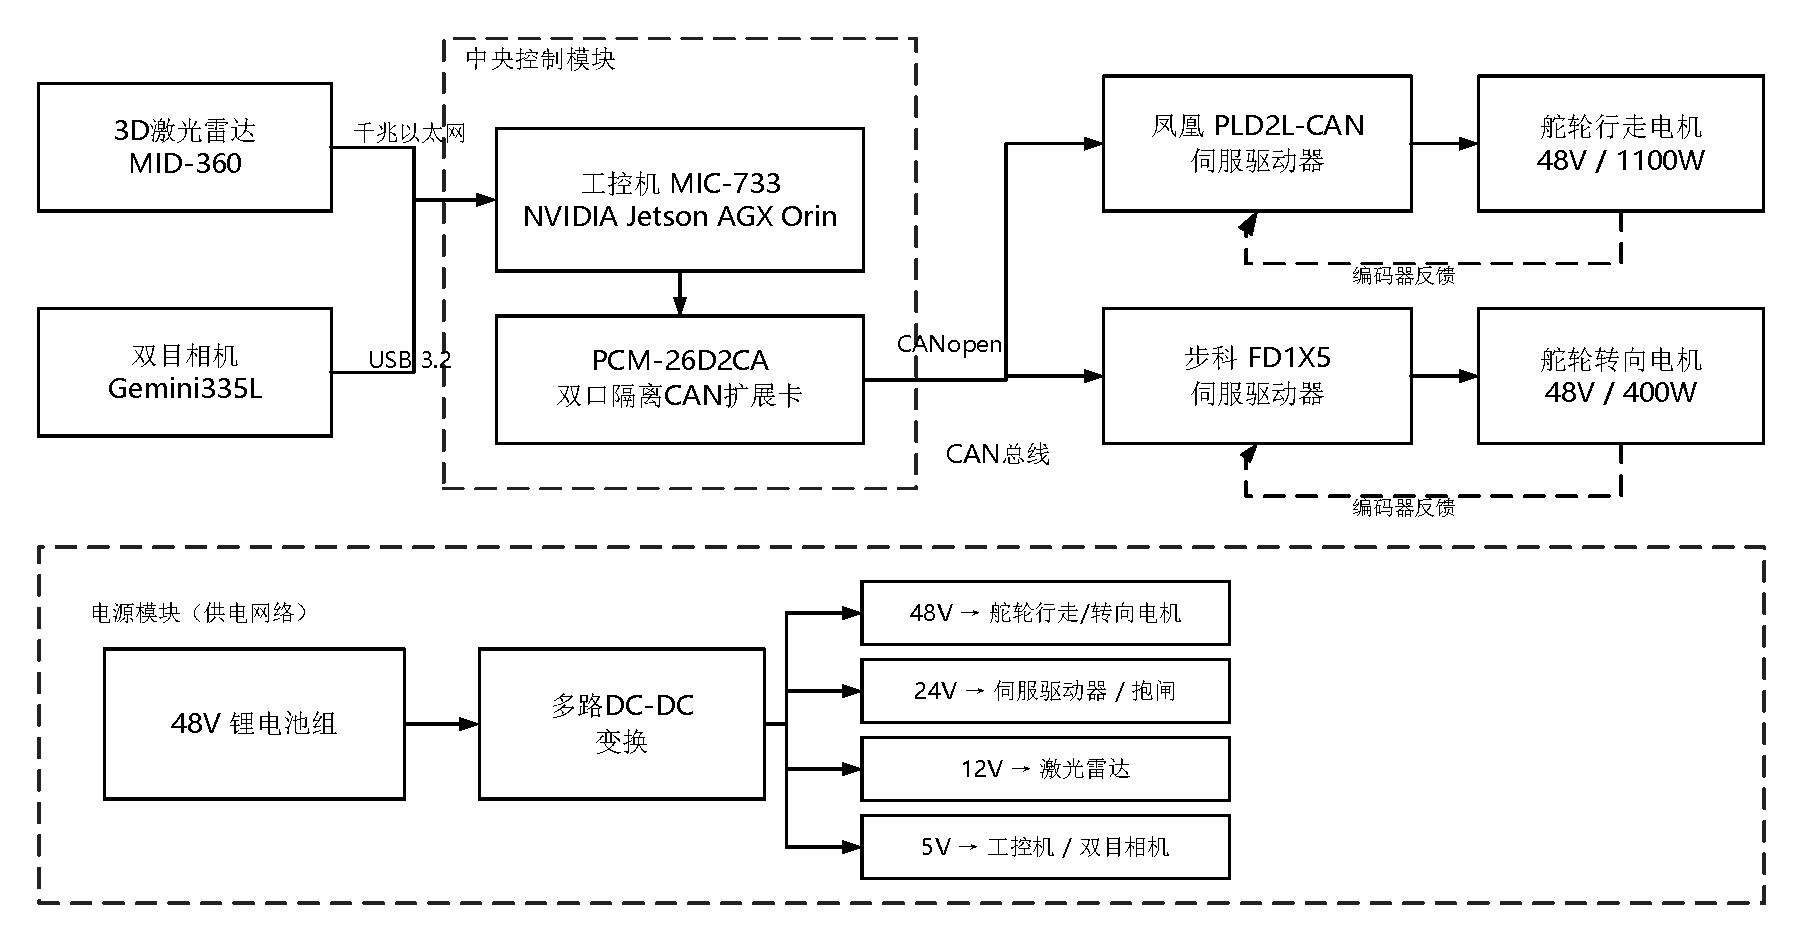
\includegraphics[width=\textwidth]{pic/硬件连接拓扑.pdf}
	\caption{机器人硬件连接拓扑}
	\label{fig:硬件连接拓扑}
\end{figure}

在感知数据链路上，MID-360激光雷达通过千兆以太网接入MIC-733的LAN口，利用PTP/PPS实现与系统时钟的硬件同步；双目相机通过USB 3.2接口连接工控机，传输RGB与深度图像数据。在控制指令链路上，工控机经Mini PCIe扩展的PCM-26D2CA双口CAN卡引出两路隔离CAN总线，分别连接行走电机驱动器（凤凰PLD2L-CAN）和转向电机驱动器（步科FD1X5）。CAN总线采用主从结构，工控机作为主站周期性下发速度与位置指令，驱动器作为从站执行指令并反馈电机状态，总线终端按规范配置120\,$\Omega$终端电阻以保证通信质量。在能量供给链路上，48V锂电池组经配电单元和DC-DC变换为各部件分配相应电压等级的电源。通过上述连接方式，各模块在统一的硬件框架下协同工作，为软件系统的运行提供物理基础。

\section{机器人软件系统架构}
机器人软件系统基于机器人操作系统（Robot Operating System, ROS）构建，运行于Ubuntu 20.04操作系统与ROS Noetic发行版之上。ROS采用分布式节点架构，各功能模块以独立节点（Node）形式运行，节点之间通过话题（Topic）、服务（Service）和动作（Action）等机制进行消息通信，并借助参数服务器和坐标变换（TF）工具统一管理系统参数与多坐标系关系。这种松耦合的设计使感知、定位、规划和控制等模块能够独立开发、测试与替换，便于系统的迭代与维护。机器人软件系统总体架构如图~\ref{fig:软件系统架构}所示，自下而上可划分为传感器驱动层、感知与定位层、规划决策层和运动控制层四个层次。

\begin{figure}[!htb]
	\centering
	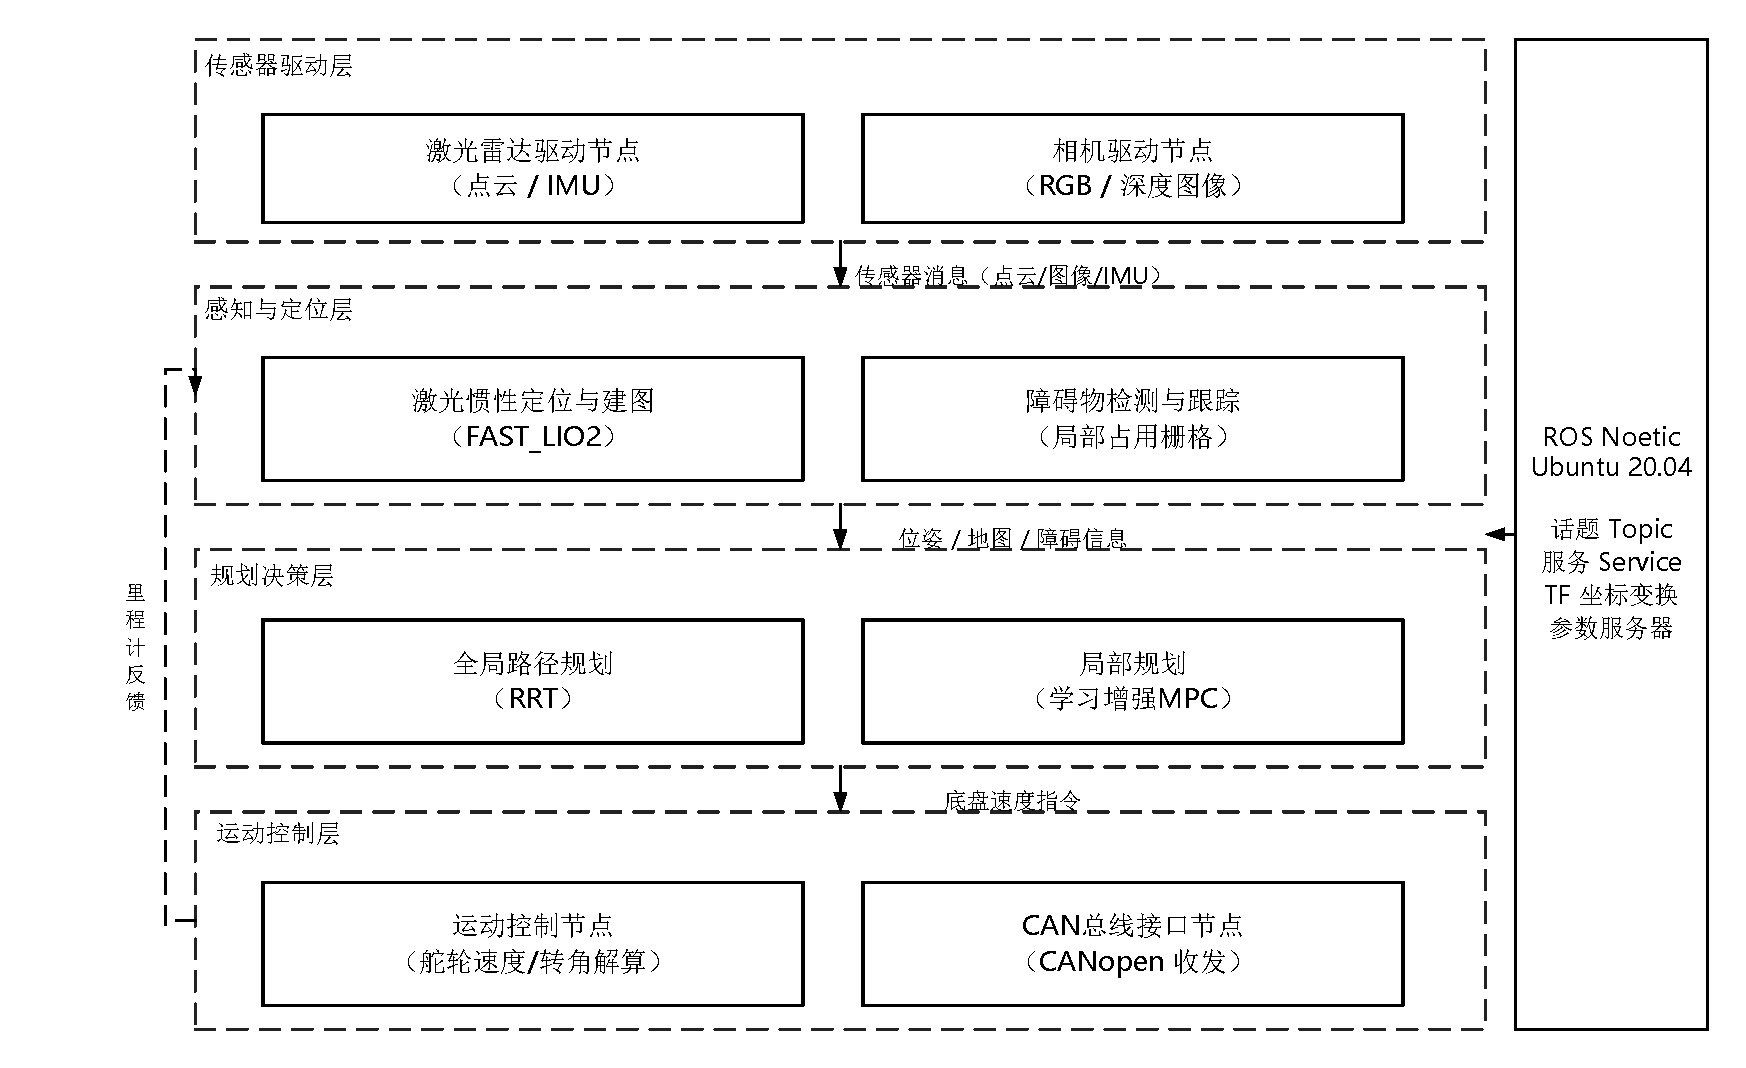
\includegraphics[width=0.92\textwidth]{pic/软件系统架构.pdf}
	\caption{机器人软件系统架构}
	\label{fig:软件系统架构}
\end{figure}

传感器驱动层负责采集并发布原始传感器数据。激光雷达驱动节点发布三维点云与IMU数据，相机驱动节点发布RGB图像与深度图像，各驱动节点将数据封装为标准ROS消息（如\texttt{sensor\_msgs/PointCloud2}、\texttt{sensor\_msgs/Image}、\texttt{sensor\_msgs/Imu}）并以话题形式向上层发布，为后续处理提供统一的数据输入。

感知与定位层是环境理解的核心。该层包含激光惯性定位建图节点和障碍物检测跟踪节点：前者基于FAST\_LIO2算法融合点云与IMU数据，在预建地图坐标系下输出机器人的全局位姿与里程计信息；后者融合深度图像与点云数据，检测并跟踪环境中的静态与动态障碍物，输出障碍物包围盒与状态估计结果，同时维护局部占用栅格地图。该层输出的位姿、地图和障碍信息为规划决策提供环境约束。

规划决策层根据导航任务和环境信息生成运动轨迹。全局规划节点基于预建地图和目标点，采用RRT算法生成全局参考路径；局部规划节点以全局路径为参考，融合实时障碍信息，通过学习增强MPC在滚动时域内求解满足运动学约束、平滑约束和避障要求的局部轨迹，并输出底盘速度指令。

运动控制层负责将速度指令转化为电机执行动作。运动控制节点将规划层输出的底盘速度指令分解为各舵轮的行走速度与转向角度，通过CAN总线接口节点按CANopen协议下发至伺服驱动器，并接收编码器反馈，实现底盘运动的闭环控制。

上述四层结构与硬件平台一一对应，数据自下而上逐层抽象、指令自上而下逐层细化，共同构成功能完整、层次清晰的机器人导航软件系统。

\section{本章小结}
本章面向变电站运维机器人的应用需求，完成了机器人系统框架的总体设计。首先，结合变电站高安全性、高可靠性和复杂空间约束的特点，分析了机器人在环境感知、定位建图、自主导航和动态避障四个方面的功能需求。其次，提出了”感知--决策--执行”的分层模块化系统方案，明确了传感器模块、中央控制模块、底层运动控制模块和电源模块的职责划分与协作关系。在此基础上，完成了硬件平台选型：感知模块选用MID-360激光雷达和Gemini335L双目相机，中央控制模块选用基于NVIDIA Jetson AGX Orin的研华MIC-733计算机并扩展CAN接口，底层运动控制模块选用凤凰动力PH210DS卧式舵轮，并分别为行走电机和转向电机配套凤凰PLD2L-CAN和步科FD1X5伺服驱动器，电源模块采用48V锂电池配合多路DC-DC变换的供电架构。随后，阐述了各部件之间的硬件连接拓扑与信号交互关系。最后，基于ROS设计了由传感器驱动层、感知与定位层、规划决策层和运动控制层构成的软件系统架构。本章设计的软硬件框架为后续各章的定位、感知与路径规划算法研究提供了统一的实现平台。


